%===================================== CHAP 5 =================================

\chapter{Phase 1: The First Prototype}
\label{chap:phase1}

\section{Exploration and Planning}
The fist phase of this project required extensive experimentation and planning as the use of VR technology with collaboration and how it can contribute to the experience of young job seekers is a relatively unexplored area of research. The primary objective for this phase was implementing a immersive and collaborative experience, but how this was to be achieved needed exploration and prototyping. As the aim for this project is to evaluate the collaborative workplace training in VR it first and foremost must support a collaborative environment in the VR world. This meant we had to implement multiplayer capability into existing workplace simulations from the ongoing project financed by NAV. It was decided that we would use Photon Unity Networking (PUN) \cite{PUN} as it enhances features built into Unity's built-in networking and UNet (Unity's multiplayer framework) will become deprecated within 2021.               

\subsection{Researchers' Night 2019}
As for the last 15 years NTNU has hosted \textit{Researchers' Night} (the youths research night) as part of a an initiative throughout Europe launched in 2005 as a means to educate and invite the youth inside the research that takes place. NTNU invited students and teachers from upper secondary and adult education institutions from Trøndelag. The IMTEL lab was present with VR and AR application tryouts and during the testing and talks we conducted a questionnaire with the aim of gathering preliminary data and opinions in relation to VR and collaboration with the respect to workplace training, see Figure \ref{fig:phase1RNGroup}. The reasoning to choosing this quantitiave data gathering method was justified by several aspects. First, quantity offers more universal means and criteria for evaluating key points and making generalised conclusions based on the result set \cite{oates2005researching}. Also, predefined answers (eg. closed answers) makes the questionnaire easy to complete for participants.

\begin{figure}[!h]
    \centering
    \captionsetup{width=.8\linewidth}
    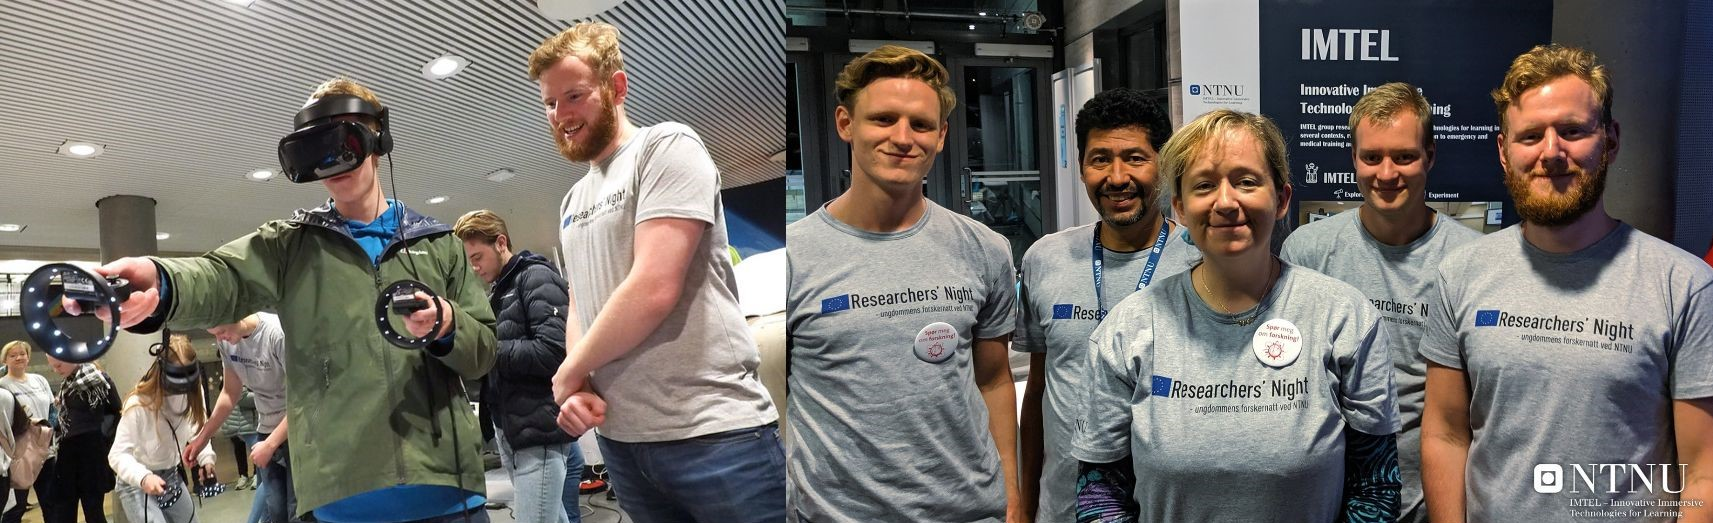
\includegraphics[width=.9\textwidth]{./fig/phase_1/researcherNight/RN_group.jpg}
    \caption{Researchers' Night 2019 showing the testing of VR application in action and group members from the IMTEL lab.}
    \label{fig:phase1RNGroup}
\end{figure}


\subsubsection{The questionnaire}
The questionnaire was comprised of two sections, one with general questions with age, sex and career guidance at school. The second contained questions aimed towards VR and the IMTEL labs' job applications (note that all participants did try a VR application before answering the questionnaire). It was generated using Google Forms \footnote{https://docs.google.com/forms/} an easy and useful questionnaire tool. Most questions where closed questions meaning they had pre-defined answers. We constructed the questionnaires in such a way that it produced both nominal, ratio and ordinal data. Most significant questions was ordinal on a consistent ranked/scale questions where the participants were asked to rank their agreement from  "Strongly disagree" to "Very agree" on a scale from 1-5. 
The full questionnaire can be found in the appendix \textcolor{red}{ADD TO APPENDIX}. 

\subsubsection{Analysis}
The questionnaire had 27 answers consisting of 78\% males and 22\%women with age distribution from 13-32. The mode being 16 years with 37\% of the participants. The data results is presented in bar and pie charts using Google Forms own utilities. There was a general agreement amongst the responds that collaborating with peers and mentors would enhance the career guidance. 77\% respondents ranked 4 and 5 (on a scale of 1-5) that they strongly agree that having peers would be beneficial, see Figure \ref{fig:phase1RNPeer}.    

\begin{figure}[!h]
    \centering
    \captionsetup{width=.7\linewidth}
    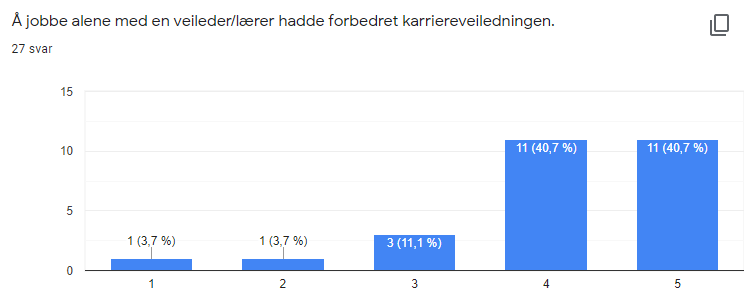
\includegraphics[width=.8\textwidth]{./fig/phase_1/researcherNight/RN_careerguidenceMentor.PNG}
    \caption{Bar chart showing the participants answers with the statement "Having a similar aged peer would enhance career guidance".}
    \label{fig:phase1RNPeer}
\end{figure}

Figure \ref{fig:RN_Apps} show the distribution of the applications which participants tried during their visit at the IMTEL lab stand.  In regards to the use of these VR applications in relation to career guidance the participant mostly agreed that they should be a part of the guidance at school, see Figure \ref{fig:RN_careerguidenceSchool}. None of the participants ranked their agreement below 3 (out of 1-5, see Figure \ref{fig:RN_VRpeer}) when asked about having a fellow peer in the VR application and that it could be beneficial. Also, 85,2\% agreed with 4 and 5 (out of 1-5) that having a mentor or teacher in the VR application could also be beneficial, the mode being a rank 5 (51,9\%).
This shows that the participants (comprised mostly of students at upper secondary school) agree that the use of VR can be beneficial in career guidance gives them a taste of different jobs and that having multiple (both peers and mentors) players can enhance the learning outcome and thus the experience. Based on evidence from this questionnaire it is clear that this is an instating field of study and it has gives us gives insight and thus motivation. However, we must also consider the limitations of this questionnaire which falls a bit short in regards to the number of participants and has almost but not correct research target audience in respect to age and education. That being said this questionnaire was only meant as preliminary data collection for for understanding and getting an overview of the field.          

\begin{figure}[!h]
    \centering
    \captionsetup{width=.6\linewidth}
    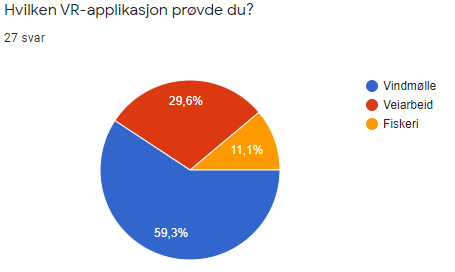
\includegraphics[width=.6\textwidth]{./fig/phase_1/researcherNight/RN_Apps.PNG}
    \caption{Pie chart showing the distribution of the applications which participants tried during their visit at the IMTEL lab stand including Fishfarm, Windmill and Construction. }
    \label{fig:RN_Apps}
\end{figure}

\begin{figure}[!h]
    \centering
    \captionsetup{width=.7\linewidth}
    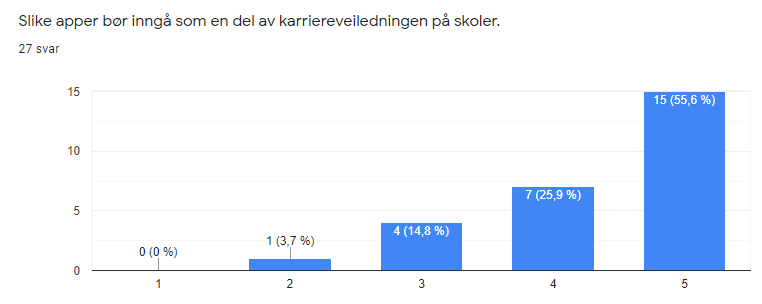
\includegraphics[width=.8\textwidth]{./fig/phase_1/researcherNight/RN_careerguidenceSchool.PNG}
    \caption{Bar chart showing the participants answers with the statement "Such applications should be a part of the career guidance at school".}
    \label{fig:RN_careerguidenceSchool}
\end{figure}

\begin{figure}[!h]
    \centering
    \captionsetup{width=.7\linewidth}
    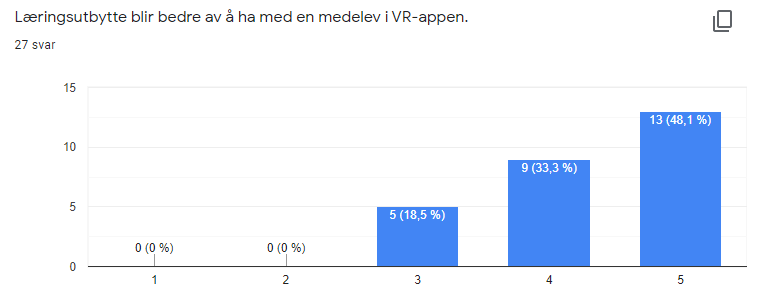
\includegraphics[width=.8\textwidth]{./fig/phase_1/researcherNight/RN_VRpeer.PNG}
    \caption{Bar chart showing the participants answers with the statement "Learning outcome is greater when having a fellow peer in the VR application".}
    \label{fig:RN_VRpeer}
\end{figure}

\subsection{Requirements}

As discussed in section \ref{sec:designCreationResearch}, the design and creation research method was selected as the most fitting way to conduct this project. As such, there was a need to gather information on user needs and specific information abut the problem. Through early conversations with the stakeholders, in this case NAV and the IMTEL lab, the most important user needs were discovered. 

After sitting down and discussing the acquired information, a few key decisions were made regarding what was needed, what was possible and what was wanted.  At the core of the project is the desire to incorporate multi-user experiences to see whether it is helpful or not to the goals of NAV. It was also important that the application could fit into their workflow and setups, as it was unrealistic that every NAV office had the space for two full VR spaces, necessitating the inclusion of a desktop mode that would allow the mentor to interact with the user from within the same virtual space, even if there only was one VR station. 

The final core need for phase 1 is angled more toward the needs of the IMTEL lab. Should it be the case that the multiplayer component is something they wish to bring forward to new workplaces they develop, a general framework or set of guidelines for multiplayer that they can build upon is wanted. With this framework/set of guidelines, a new workplace could be made to work with multiplayer from the get go, drastically reducing the amount of work needed to get multiplayer running for future projects.

This lead to the following functional requirements for phase 1. 

\begin{enumerate}
  \setlength\itemsep{0em}
  \item [\textbf{F1}] The applications must allow multiple players to join the same scene.
  \item [\textbf{F2}] Interactable objects must be serialised and and synchronised over the network.
  \item [\textbf{F3}] A player shall be represented as a avatar with corresponding movement from the real world to the VR world.
  \item [\textbf{F4}] The application must offer the option of using VR equipment or desktop mode (mouse and keyboard) for interaction.
  \item [\textbf{F5}] The application must contain a scene with tasks enabling collaborative learning.
  \item [\textbf{F6}] The multiplayer component must be generalisable and scalable to work with other NAV applications.
\end{enumerate}

\subsection{Development decisions}
\subsubsection{Choice of development platform}
Since one of the purposes of the project was to heighten the quality and experience of the existing applications developed at the IMTEL lab, the choice of development platform was already locked in. As the project had used Unity before, we opted to continue doing exactly that.





\section{Implementation}

\subsection{Implementing VR in Unity}
When it comes to developing for VR in Unity, there are numerous tools available. Drawing upon the expertise of the IMTEL lab and discussion with previous master degree students, as well as reading previous IMTEL papers, the choice was made to use SteamVR \cite{steamVR}\cite{steamVRAPI}. By targeting SteamVR for development, the application will automatically work on a large range of the most commonly used headsets without needing any further effort from the developer side. When programming, one uses words like grab and pinch to define the action instead of mapping and action directly to a certain input. SteamVR will then translate that to the correct action for the end user, regardless of what type of controller they're using, so long as it is SteamVR compatible.

\subsubsection{Movement}
Movement in VR is primarily achieved through two methods. Physical motion of the body in the play area, as well as \textit{teleportation} inside the game. Due to a limited physical area, it becomes necessary to combine these two forms to move efficiently in VR. Teleport for long distances, physical movement for minute and precision movement. Using the SteamVR plug-in for Unity\cite{steamVRAPI}, this can all be handled with relative ease. However, due to the inclusion of Photon networking, it becomes necessary to translate these movements onto another object, one which can be networked to other players. 

The Steam VR player object functions as a singleton. This means that there can only ever be one of them in any one instance. Many of the key interaction systems of Steam VR rely on there only ever being one Player object, and never more than that. For collaborative purposes, we need more than one player. Therefore, an avatar representing the player is created. This is invisible to the player, but is shown to the other players as it copies whatever the user does. In this way, we can always use the singleton Player object on each client, while still showing all the users' movements and actions simultaneously to everyone currently in the room. 

\subsubsection{Interactable Objects}
When working with Photon, numerous features are abstracted and automated. For developers, it becomes a question of figuring out what needs to be networked, and what doesn't. By adding a few components to a game object, and instantiating it through Photon's systems rather than Unity's instantiation systems, Photon can track the object's state and synchronise it across all users. The last player to interact with an object becomes it's \textit{owner}, the truth source of this particular object. Therefore, once an object is in the hand of a user, other players can observe the actions of the user and the effect on the object.

\subsection{Issues}

\subsubsection{Ownership transfer of interactable objects}
We experienced issues related to the SteamVR player and Photon Transform view. We could transfer objects to each other but the previous owner would not see the other user take the object from their hand until they let go of it, of which there is no clear indication that they must do, aside from some minor jittering of the object.

\subsubsection{Git and LFS for Unity}
\textcolor{red}{Crashing while using Git, Unity and PUN}

\subsubsection{Uncanny valley; representing the player as humanoids}
In the first phase, simple low-poly human heads were used for the avatars representing the users, along with a capsule body and hands for the rest of the body. For collaborative VR, it is important to consider the effects of the \textit{uncanny valley}\cite{mori2012uncanny}. If the users feel any form of aversion due to the avatars, they may need to be changed for something less human-like. An article from 2017 by Seyama and Nagayama \cite{seyama2007uncanny} pinpointed that a realistic face is a necessary condition for triggering the \textit{uncanny valley} effect, but is not always enough by itself. Some bizarre facial feature like supersized eyes or off putting motion needs to be present as well. Since the heads of our avatars have no distinct facial features or actual animation, they may elicit no specific response at all.

\subsection{Result of phase 1 implementation}
The first phase of the project was focused on features. A plan was made concerning which collaborative features were needed for an MVP, and these were implemented in a test space made primarily for prototyping and testing purposes. This was made using a garage asset from one of the other projects of the lab, and several objects were placed into the scene with a simple corresponding task for users to interact with, see Figure \ref{fig:phase1Capture1}. While not all features that may prove useful had been implemented, enough was done that we believed a test could be performed to gauge the usefulness of the collaborative tools. 

Preferably, we hoped to get some data from the users about what features worked well, which ones didn't and other things we may have missed.


\begin{figure}
    \centering
    \captionsetup{width=.7\linewidth}
    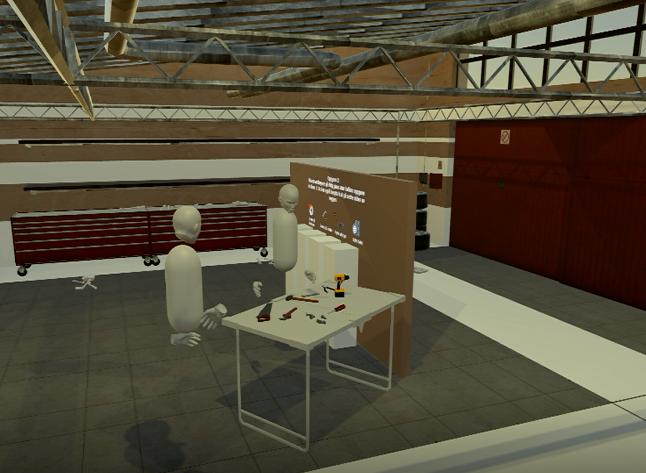
\includegraphics[width=.7\textwidth]{./fig/phase_1/phase1_capture2.PNG}
    \caption{Screencapture of the test environment showing two users using different HMDs collaborating on a task simultaneously while being connected over the network.}
    \label{fig:phase1Capture1}
\end{figure}


\section{First Evaluation}
Testing of the first prototype took place with the help of NAV. Two laptops and inside-out MR headsets were brought to a facility where we could test the prototype and interview the participants (see Figure \ref{fig:testingPhase1}). Initial results were positive, with the participants offering solid feedback. It is worth noting, however, that since the tests were conducted with the two users in the same room, it may not be completely accurate to every potential usecase of the application, such as long distance collaboration. In such cases, one would need voice chat to be functional, which it is not in the first prototype.

\begin{figure}[H]
  \centering
    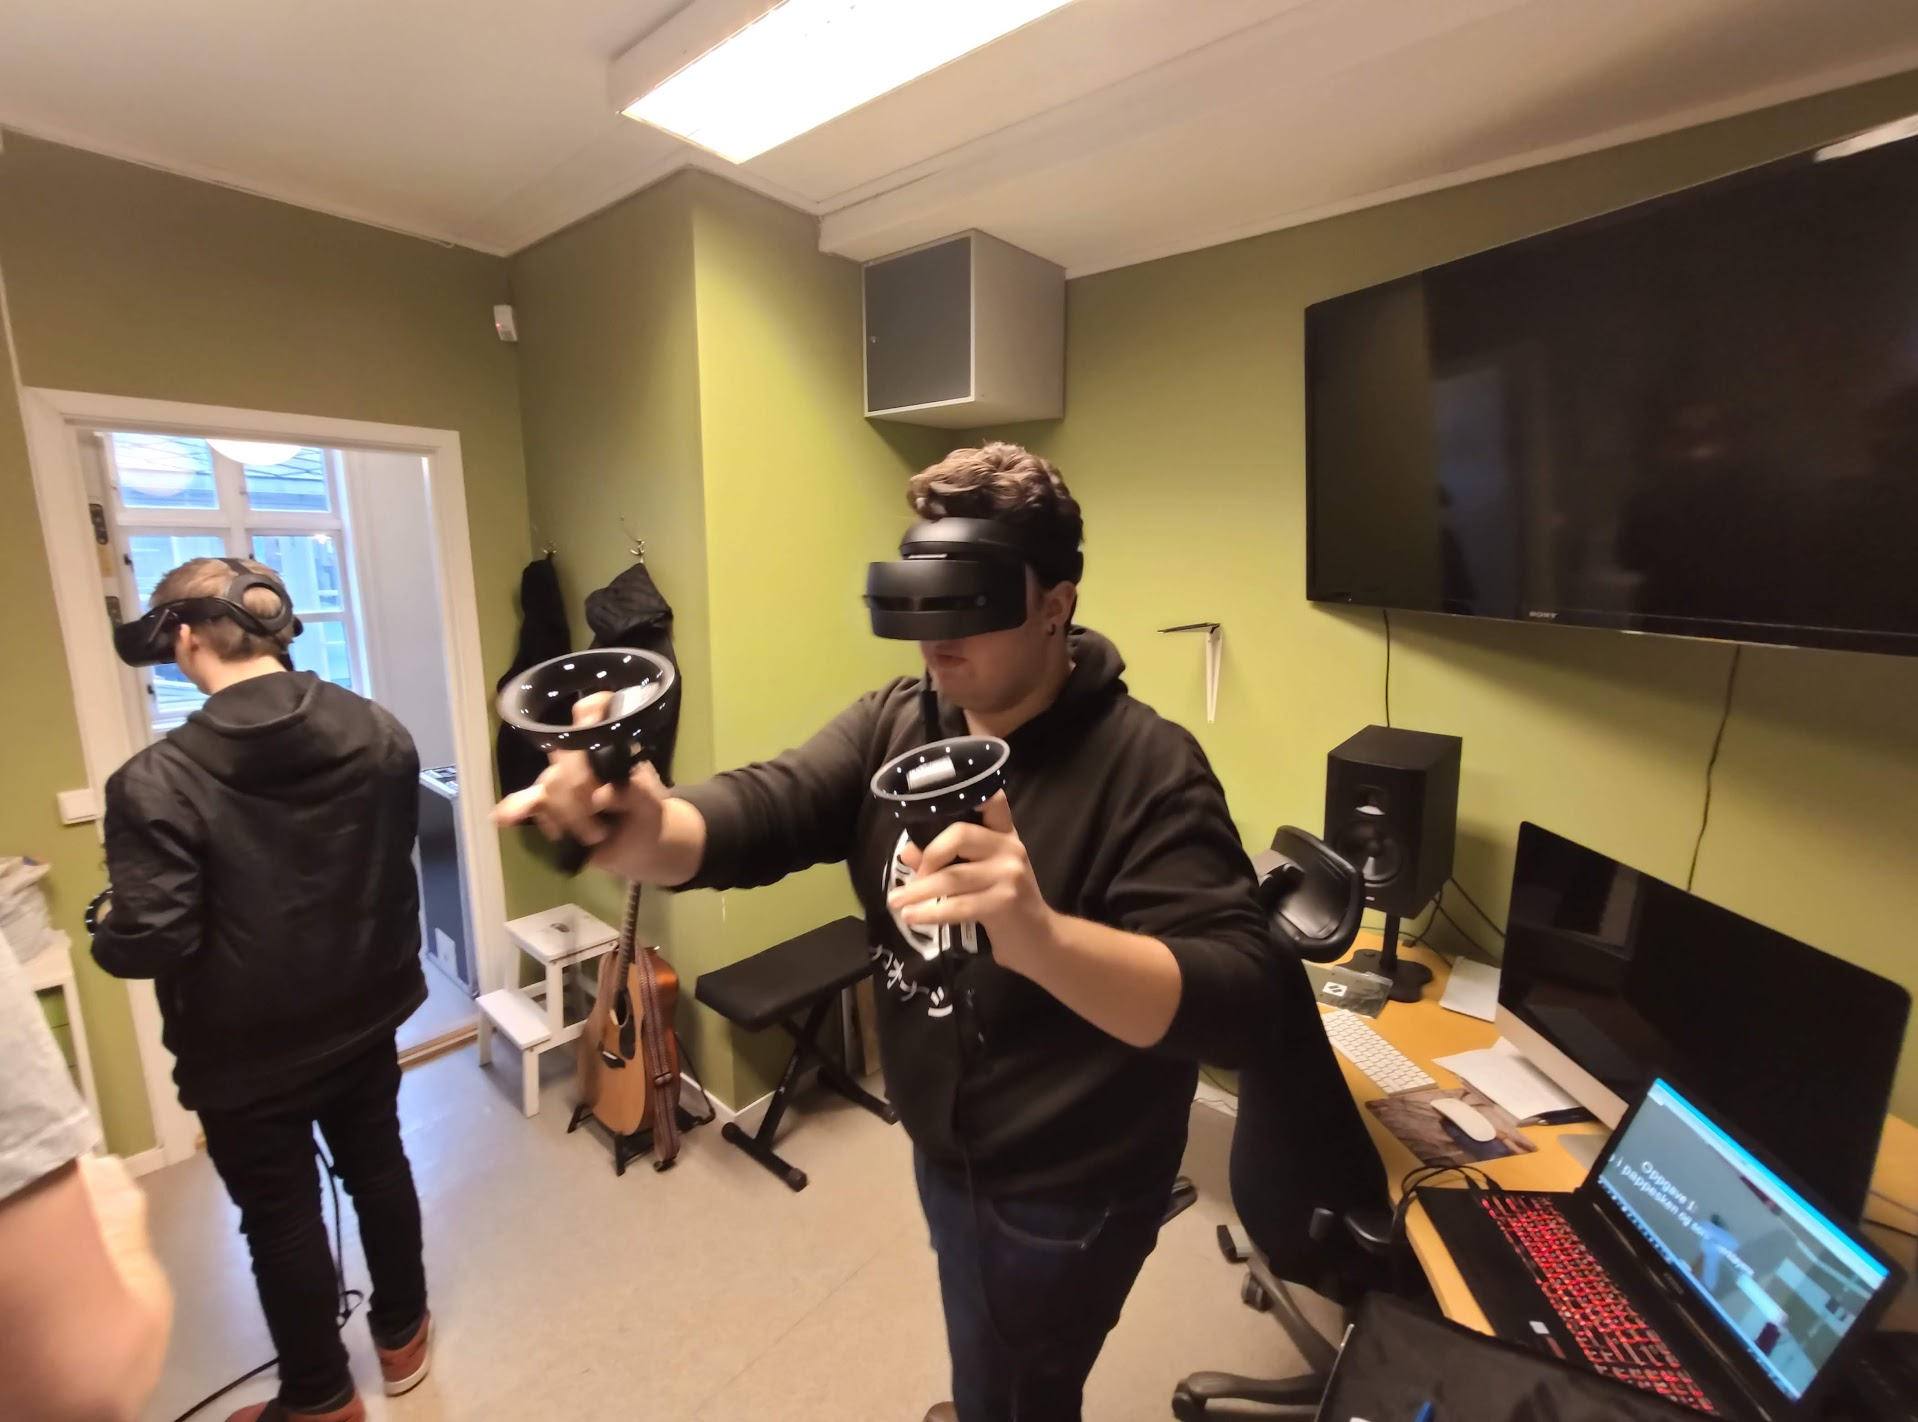
\includegraphics[width=0.7\textwidth]{fig/phase_1/testingPhase1.jpg}
 \caption{Testing in action with two primary users from NAV.}
\label{fig:testingPhase1}
\end{figure}


\subsection{User test data}

\subsection{Analysis}
\subsubsection{Qualitative Textual Data Analysis}
In order to analyse the textual data from the interviews conducted for phase 1 we utilised multiple techniques to help manage and analyse the interview materials as suggested by Oates in his book \textit{Researching Information Systems and Computing } \cite{oates2005researching}. First, we prepared the textual data by making a duplicate of the material which ensured that we did not harm our original data. Then we could ensure the same format and similar naming conventions for all data helping us to manage it. Through an inductive approach \cite{oates2005researching} we conducted \textit{theme analysis} and observed categories in the material by studying them. From there we could get a greater understanding of the feedback from the tests and evaluate the result with its limitations and achievements.

Table \ref{table:themesInterview1} shows the themes which were determined after the analysis process and their related more refined sub-themes.  Table \ref{table:methaphorsInterview1} illustrates relevant metaphors identified in the interviews by each interviewee and it was a helpful diagram to help manage the interview material. Finally, Table \ref{table:satificationInterview1} shows the interviewees satisfaction of the application presented in the test.     

\begin{table}[!h]
      \centering
        \begin{tabular}{ll}
        \toprule
        Theme & Sub-theme \\
        \midrule
        Interaction & Voice communication or voice chat\\
        & Pointing/marker \\\vspace{0.2cm}
        & Personalisation (avatar skins) \\
        Collaboration & Focus on collaborative tasks \\\vspace{0.2cm}
        & Tasks which require at least 2 players \\
        Game design & Controller guidance (toggle on/off)\\
        & Level design\\
        & Distinction between roles\\
        \bottomrule
        \end{tabular}
        \caption{The identified themes and sub-themes from the analysis.}
        \label{table:themesInterview1}
\end{table}



\begin{table}[!h]
\centering
\begin{tabular}{l|llllll}
                            & \#01 &\#02 &\#03 &\#04 & \#05 & \#06 \\ \hline 
Avatar skin                 & *        &          &          &          &          & *        \\ 
Fun                         & *        & *        &          & *        &          & *        \\ 
Engaging                    & *        &          & *        &          &          &          \\ 
Voice communication         & *        & *        &          &          &          &          \\ 
Easy                        &          &          & *        &          &          & *        \\ 
Gamification                & *        &          &          &          &          &          \\ 
Collaboration focused tasks & *        & *        & *        & *        & *        &          \\ 
Natural with multiplayer    &          &          & *        & *        & *        &          \\ 
Presence                    &          & *        & *        &          &          & *        \\ 
Controller explanation      &          &          & *        & *        &          &          \\ 
Habituation                 &          & *        &          &          & *        & *        \\ 
Pointing                    & *        & *        &          &          &          & *        \\ 
\end{tabular}

\caption{Identified metaphors/keywords from the interview material.}
\label{table:methaphorsInterview1}
\end{table}


\begin{table}[!h]
      \centering
        \begin{tabular}{llp{2.5cm}p{5cm}}
        \toprule
        Role & ID & Satisfaction with the system & Reason\\
        \midrule
         & \#01 & High & Better. More atmosphere and engaging. Fun to work.\\\vspace{0.2cm}
         & \#02  & Medium & Enhanced the experience, but need more distinct collaboration tasks.\\\vspace{0.2cm}
         Job seeker & \#03  & High & Increased presence and multiplayer seems better. Has potential and can be more engaging.\\\vspace{0.2cm}
         & \#04 & High & Positive experience, especially when more people help each other. More fun.  \\\vspace{0.2cm}
         & \#05  & Low & Stressful. Not always aware of where the other player is. Better through habituation. \\\midrule
        Mentor & \#06  & High &  Exiting to mentor the other less experienced player. Easier to give instructions as one is present in the same world. \\
        \bottomrule
        \end{tabular}
        \caption{Satisfaction of the application grouped according to the role of each interviewee.}
        \label{table:satificationInterview1}
\end{table}


\subsubsection{Interaction and realism}
A few of the participants pointed out the current choice of avatars, and there was a discussion about them. While they felt the simple grey avatars were functional, some wanted to be able to choose avatars or at least do some minor customisation, like the colour of the avatar. The interaction itself mostly felt normal, and was not intrusive. One, who was not a accustomed to VR, felt that the other person was helpful in realising what was possible and what was not, even if the avatar moved a little strangely.

\subsubsection{Visibility and simplicity}
Due to the simplicity of the avatars and the general scene, most things were relatively clear, and not too cluttered. Some reported difficulty reading the text, which may be due to the limited resolution of the MR headsets that were used for the tests. Since usability is very important, and increasing text size is quite simple, this may be done for the next version.

Worth noting is that the premade asset used to construct the test scene contains a lot of visual clutter and objects one might assume to be intractable that is not. While not directly related to collaboration, this can confuse and reduce the user's feeling of presence by reminding them of the limitations of the virtual environment. An attempt should be made to reduce visual clutter where possible, and that scenes do not contain misleading objects.

\subsubsection{Real content}


\subsubsection{Considerations for the next survey}
There was some back and forth as to what method should be used for the data gathering on the first survey, as we were not certain how many users would be present and available for testing. Therefore the constructed interview guide was slightly rushed. While we consulted with our supervisor, we need to make sure that the next survey is more properly vetted and double checked to remove any possibility of leading questions or bias. 

\subsubsection{Updated Requirements}
The requirements will stay mostly the same. An additional requirement for phase two is that voice chat must be implemented, and preferably some tools the users can use to mark or pinpoint objects or locations that they want to draw attention to.



\cleardoublepage